% **************************************************
% Document Class Definition
% **************************************************
\documentclass[%
    paper=A4,               % paper size --> A4 is default in Germany
    twoside=true,           % onesite or twoside printing
    openright,              % doublepage cleaning ends up right side
    parskip=full,           % spacing value / method for paragraphs
    chapterprefix=true,     % prefix for chapter marks
    11pt,                   % font size
    headings=normal,        % size of headings
    bibliography=totoc,     % include bib in toc
    listof=totoc,           % include listof entries in toc
    titlepage=on,           % own page for each title page
    captions=tableabove,    % display table captions above the float env
    draft=false,            % value for draft version
]{scrreprt}%


% **************************************************
% Setup YOUR thesis document in this file !
% **************************************************
% !TEX root = main.tex


% **************************************************
% Files' Character Encoding
% **************************************************
\PassOptionsToPackage{utf8}{inputenc}
\usepackage{inputenc}
\usepackage[english,ngerman]{babel}

% **************************************************
% Information and Commands for Reuse
% **************************************************
\newcommand{\thesisTitle}{Probabilistische online Wissensgraphkonstruktion aus natürlicher Sprache}
\newcommand{\thesisName}{Clemens Damke}
\newcommand{\thesisMatNr}{7011488}
\newcommand{\thesisSubject}{Bachelorarbeit}
\newcommand{\thesisDate}{\today}
\newcommand{\thesisVersion}{Entwurf 1}

\newcommand{\thesisFirstReviewer}{Prof.~Dr.~Eyke Hüllermeier}
\newcommand{\thesisFirstReviewerUniversity}{\protect{Universität Paderborn}}
\newcommand{\thesisFirstReviewerDepartment}{Institut für Informatik}

\newcommand{\thesisSecondReviewer}{Prof.~Dr.~Axel-Cyrille Ngonga Ngomo}
\newcommand{\thesisSecondReviewerUniversity}{\protect{Universität Paderborn}}
\newcommand{\thesisSecondReviewerDepartment}{Institut für Informatik}

\newcommand{\thesisFirstSupervisor}{Dr.~Theodor Lettmann}
\newcommand{\thesisSecondSupervisor}{Prof.~Dr.~Eyke Hüllermeier}

\newcommand{\thesisUniversity}{Universität Paderborn}
\newcommand{\thesisUniversityDepartment}{}
\newcommand{\thesisUniversityInstitute}{Institut für Informatik}
\newcommand{\thesisUniversityGroup}{Intelligente Systeme}
\newcommand{\thesisUniversityCity}{Paderborn}
\newcommand{\thesisUniversityStreetAddress}{Pohlweg 51}
\newcommand{\thesisUniversityPostalCode}{33098}


% **************************************************
% Debug LaTeX Information
% **************************************************
%\listfiles


% **************************************************
% Load and Configure Packages
% **************************************************

% Colors:
\usepackage[usenames, dvipsnames, svgnames, table]{xcolor}

\definecolor{blau}{HTML}{355FB3}
\definecolor{rot}{HTML}{B33535}
\definecolor{gruen}{HTML}{3BB335}
\definecolor{dunkelblau}{HTML}{1E3666}
\definecolor{hellblau}{HTML}{8ea7d7}

\PassOptionsToPackage{% setup clean thesis style
    figuresep=space,
    sansserif=false,
    hangfigurecaption=false,
    hangsection=true,
    hangsubsection=true,
    colorize=full,
    colortheme=custom,
	colormain=dunkelblau,
	coloraccessory=blau,
    bibsys=bibtex,
    bibfile=bib-refs,
    bibstyle=alphabetic,
    wrapfooter=false,
}{cleanthesis}
\usepackage{cleanthesis}

\usepackage{mathtools}
\newcommand\numberthis{\addtocounter{equation}{1}\tag{\theequation}}

\usepackage{stmaryrd}

\usepackage{tikz}
\usetikzlibrary{calc}
\newcommand{\tikzmark}[1]{\tikz[overlay,remember picture] \node (#1) {};} % chktex 1

\usepackage[bguq]{frege}

\usepackage{pgfplots}
\usepackage{pgfplotstable}
\pgfplotsset{compat=1.14}
\usepgfplotslibrary{dateplot, statistics}
\pgfplotsset{
    cycle list={blau\\rot\\gruen\\},
}

\hypersetup{% setup the hyperref-package options
    pdftitle={\thesisTitle},    %   - title (PDF meta)
    pdfsubject={\thesisSubject},%   - subject (PDF meta)
    pdfauthor={\thesisName},    %   - author (PDF meta)
    plainpages=false,           %   -
    colorlinks=false,           %   - colorize links?
    pdfborder={0 0 0},          %   -
    breaklinks=true,            %   - allow line break inside links
    bookmarksnumbered=true,     %
    bookmarksopen=true          %
}



% **************************************************
% Document CONTENT
% **************************************************
\begin{document}

% --------------------------
% rename document parts
% --------------------------
\renewcaptionname{ngerman}{\figurename}{Abb.}
\renewcaptionname{ngerman}{\tablename}{Tab.}
%\renewcaptionname{english}{\figurename}{Fig.}
%\renewcaptionname{english}{\tablename}{Tab.}

% --------------------------
% Front matter
% --------------------------
\pagenumbering{roman}			% roman page numbing (invisible for empty page style)
\pagestyle{empty}				% no header or footers
% !TEX root = ../main.tex
%
% ------------------------------------  --> cover title page
\begin{titlepage}
	\pdfbookmark[0]{Cover}{Cover}
	\flushright\
	\hfill
	\vfill
	{\LARGE\thesisTitle\ \par}
	\rule[5pt]{\textwidth}{.4pt} \par
	{\Large\thesisName}
	\vfill
	\textit{\large\thesisDate} \\
	Version: \thesisVersion\
\end{titlepage}


% ------------------------------------  --> main title page
\begin{titlepage}
	\pdfbookmark[0]{Titlepage}{Titlepage}
	\tgherosfont\

	\begin{figure}
	\begin{minipage}[t]{8.5cm}
	
\includegraphics[height=1.8cm]{gfx/upb_1E}\\
	\textsf{\small{\hspace*{1.3cm}Department of Electrical Engineering,\\
	\hspace*{1.3cm}Computer Science and Mathematics\\
%		\hspace*{1.3cm}Institute of Computer Science\\
		\hspace*{1.3cm}Warburger Straße 100 \\
		\hspace*{1.3cm}33098 Paderborn
		}}
	\end{minipage}
	\hfill
	\begin{minipage}[t]{4.7cm}
	
\includegraphics[height=1.8cm]{gfx/is-logo-klein}\\
	\textsf{%Institute of Computer Science\\
	\hspace*{0.1cm}\small{Intelligent Systems Group (ISG)}
	}
	\end{minipage}
	\end{figure}

	\centering
	%\textsf{\thesisUniversityDepartment} \\
	%\textsf{\thesisUniversityInstitute} \\
	%\textsf{\thesisUniversityGroup} \\

	\vfill
	{\large \thesisSubject} \\[5mm]
	{\LARGE \color{ctcolortitle}\textbf{\thesisTitle} \\[10mm]}
	{\Large \thesisName} \\

	\vfill
	\begin{minipage}[t]{.27\textwidth}
		\raggedleft\
		\textit{1. Korrektor}
	\end{minipage}
	\hspace*{15pt}
	\begin{minipage}[t]{.65\textwidth}
		{\Large \thesisFirstReviewer} \\
	  	{\small \thesisFirstReviewerDepartment} \\[-1mm]
		{\small \thesisFirstReviewerUniversity}
	\end{minipage} \\[5mm]
	\begin{minipage}[t]{.27\textwidth}
		\raggedleft\
		\textit{2. Korrektor}
	\end{minipage}
	\hspace*{15pt}
	\begin{minipage}[t]{.65\textwidth}
		{\Large \thesisSecondReviewer} \\
	  	{\small \thesisSecondReviewerDepartment} \\[-1mm]
		{\small \thesisSecondReviewerUniversity}
	\end{minipage} \\[10mm]
	\begin{minipage}[t]{.27\textwidth}
		\raggedleft\
		\textit{Betreuer}
	\end{minipage}
	\hspace*{15pt}
	\begin{minipage}[t]{.65\textwidth}
		\thesisFirstSupervisor\ und \thesisSecondSupervisor\
	\end{minipage} \\[10mm]

	\thesisDate\\ % chktex 21

\end{titlepage}


% ------------------------------------  --> lower title back for single page layout
\hfill
\vfill
{
	\small
	\textbf{\thesisName} \\
	\textit{\thesisTitle} \\
	\thesisSubject, \thesisDate\\ % chktex 21
	Korrektoren: \thesisFirstReviewer\ und \thesisSecondReviewer\\ % chktex 21
	Betreuer: \thesisFirstSupervisor\ und \thesisSecondSupervisor\\[1.5em] % chktex 21
	\textbf{\thesisUniversity} \\
	\textit{\thesisUniversityGroup} \\
	\thesisUniversityInstitute\\ % chktex 21
	\thesisUniversityDepartment\\ % chktex 21
	\thesisUniversityStreetAddress\\ % chktex 21
	\thesisUniversityPostalCode\ \thesisUniversityCity\
}
		% INCLUDE: all titlepages
\cleardoublepage

\pagestyle{plain}				% display just page numbers
% !TEX root = ../my-thesis.tex
%
\pdfbookmark[0]{Abstract}{Abstract}
\chapter*{Abstract}
\label{sec:abstract}
\vspace*{-10mm}

\blindtext

\vspace*{20mm}

{\usekomafont{chapter}Abstract (different language)}\label{sec:abstract-diff} \\

\blindtext
		% INCLUDE: the abstracts (english and german)
\cleardoublepage
%
% !TEX root = ../my-thesis.tex
%
\pdfbookmark[0]{Acknowledgement}{Acknowledgement}
\chapter*{Acknowledgement}
\label{sec:acknowledgement}
\vspace*{-10mm}

\Blindtext[2][2]
 % INCLUDE: acknowledgement
\cleardoublepage
%
\setcounter{tocdepth}{2}		% define depth of toc
\tableofcontents				% display table of contents
\cleardoublepage

% --------------------------
% Body matter
% --------------------------
\pagenumbering{arabic}			% arabic page numbering
\setcounter{page}{1}			% set page counter
\pagestyle{maincontentstyle} 	% fancy header and footer

% !TEX root = ../main.tex
% chktex-file 46
\chapter{Einleitung}%
\label{sec:intro}

\cleanchapterquote{
The actual world cannot be distinguished from a world of imagination by any description.
Hence the need of pronoun and indices, and the more complicated the subject the greater the need of them.
}{Charles Sanders Peirce}{Mathematiker und Philosoph}

\section{Motivation}%
\label{sec:intro:motivation}

In den letzten Jahren hat die Repräsentation von Wissensbasen durch Graphen, sog. Wissensgraphen, immer mehr an Bedeutung gewonnen.
Google, Bing und IBM Watson benutzen solche Wissensgraphen z.~B. zum Beantworten von komplexen Suchanfragen.

Die Grundidee dabei ist es, Entitäten durch Knoten und Relationen durch Kanten abzubilden.
Entitäten können konkrete Dinge, wie z.~B. Personen, aber auch abstrakte Konzepte, wie z.~B. historische Epochen, sein.
Relationen beschreiben beliebige Beziehungen zwischen den Entitäten, z.~B. $person(\text{Da~Vinci}) \xrightarrow{\text{lived~in}} epoch(\text{Renaissance})$.
Die Entität, von der eine solche Relation ausgeht, wird als Subjekt und die Zielentität als Objekt der Relation bezeichnet.

Die Typen von Entitäten bzw.\ Relationen (z.~B. $person$ bzw. $lived~in$) und deren Bedeutung sind dabei i.~d.~R. formal in einer sog.\ Ontologie spezifiziert.
Die Ontologie beschränkt also die Menge gültiger Wissensgraphen, was eine effiziente maschinelle Verarbeitung der im Graph enthaltenen Informationen ermöglicht.

Da Wissensgraphen in zahlreichen Domänen einsetzbar sind, wird deren automatisierte Konstruktion bereits seit Jahren erforscht.
Manuelles Konstruieren und vor allem anschließendes Warten und Aktualisieren von Wissensgraphen, ist aufgrund der abzubildenden Datenmengen nicht praktikabel.
Bei einer maschinellen automatisierten Konstruktion sind insbesondere zwei Anforderungen problematisch:
\begin{enumerate}
	\item Das Verarbeiten von unstrukturierten Eingaben, wie z.~B. natürlichsprachlichen Texten.
	\item Effizientes Eingliedern neuer Informationen in einen bestehenden Wissensgraphen.
		Dieses Eingliedern von Informationen umfasst im Speziellen:
		\begin{itemize}
			\item \textbf{Entity Resolution:}
				Hinzukommende Entitäten, die bereits im Graphen enthalten sind, müssen als Duplikate erkannt werden.
				Dies ist i.~d.~R. nicht trivial, da die selbe Entität durch viele verschiedene, oftmals vom Kontext abhängige, Token repräsentiert werden kann;
				z.~B. \textit{Bob} vs. \textit{Robert} oder \textit{Der Papst} vs. \textit{Franziskus}.
			\item \textbf{Link Prediction:}
				Hinzukommende Entitäten müssen mit bereits bestehenden Entitäten in Relation gesetzt werden.
				Hinzukommende Relationen können zudem benutzt werden um andere Relationen zu inferieren;
				z.~B. \[female(A) \land B \xrightarrow{\text{son~of}} A \implies A \xrightarrow{\text{mother~of}} B\]
		\end{itemize}
\end{enumerate}

Die Kombination dieser beiden Anforderungen ist interessant, da das meiste verfügbare Wissen in natürlichsprachlicher Textform vorliegt und zudem permanent neues Wissen entsteht.
Ein automatisiertes Wissensgraphkonstruktionsverfahren, welches beide Anforderungen berücksichtigt, ist daher in diversen Domänen von Nutzen.
Ein Beispiel hierfür ist die Auswertung von Kommunikationsdaten aus E-Mails oder Chat-Nachrichten mit dem Ziel die sozialen Beziehungen und Intentionen der Kommunikationpartner zu ermitteln.

\section{Ziele der Arbeit}%
\label{sec:intro:goals}

Das übergeordnete Ziel dieser Arbeit ist es, ein Verfahren zu finden, welches das soeben beschriebene Problem der automatisierten Wissensgraphkonstruktion für E-Mail-Daten löst.
Konkret sei ein Stream von E-Mails gegeben, denen jeweils ein Inhalt, ein Absender, eine Menge von Empfängern und ggf.\ weitere Metadaten, wie z.~B. Absendezeit, Absendeort oder IP-Adresse, zugeordnet ist.
Die Nachrichteninhalte werden der Einfachheit halber als ausschließlich englischsprachig angenommen.
Außerdem wird eine, für E-Mails und andere Kurznachrichten typische, eingeschränkte Sprachkomplexität angenommen.
Die Nachrichten sollen nacheinander in das zu konstruierende System eingefügt werden, welches sukzessive einen Wissensgraphen daraus erzeugt.

Für diese Erzeugung muss eine Reihe von Teilproblemen gelöst werden:
\begin{enumerate}
	\item \textbf{Onotologie:}
		Spezifikation einer Wissensgraphontologie, die mächtig genug ist, um die Diversität natürlichsprachlich beschriebener Informationen abzubilden.
	\item \textbf{Repräsentation:}
		Spezifikation der maschinellen Repräsentation des Wissensgraphen.
	\item \textbf{Sprachverarbeitung:}
		Finden eines Verfahrens, welches die natürlichsprachlichen Inhalte der Nachrichten in eine für die Wissensgraphkonstruktion geeignete Form bringt.
	\item \textbf{Grapherweiterung:}
		Finden eines Verfahrens, um eine eintreffende Nachricht in den bestehenden Wissensgraphen einzufügen.
\end{enumerate}

Das aus den Teillösungen zusammengesetzte Verfahren muss, neben der offensichtlichen Anforderung einen Wissensgraphen zu konstruieren, zudem folgende technische Anforderungen erfüllen:
\begin{enumerate}
	\item \textbf{Erweiterbarkeit:}
		Es sollen Schnittstellen eingeplant sein, um neben der Sprachverarbeitung auch andere Verarbeitungsverfahren, z.~B. für Bilder, hinzufügen zu können.
		Die Graphontologie, Graphrepräsentation und das Grapherweiterungsverfahren dürfen also nicht zu sehr auf die Struktur natürlicher Sprache zugeschnitten sein.
	\item \textbf{Parallelisierbarkeit:}
		Das Verfahren soll in der Lage sein die Rechenleistung mehrerer Prozessorkerne zu nutzen.
		Diese Anforderung betrifft insbesondere das Grapherweiterungsverfahren.
\end{enumerate}

\section{Aufbau der Arbeit}%
\label{sec:intro:structure}

\paragraph{Kapitel~\ref{sec:related}}

\paragraph{Kapitel~\ref{sec:theory}}

\paragraph{Kapitel~\ref{sec:text2kg}}

\paragraph{Kapitel~\ref{sec:evaluation}}

\paragraph{Kapitel~\ref{sec:conclusion}}
   % INCLUDE: introduction
% !TEX root = ../main.tex
% chktex-file 46
\chapter{Verwandte Arbeiten}%
\label{sec:related}

Die in~\ref{sec:intro:goals} beschriebenen Ziele werden bereits seit langem erforscht.
Der Begriff \textit{Wissensgraph} wurde 2012 durch Google popularisiert, die Ideen dahinter lassen sich allerdings bis ins Ende des 19. Jahrhunderts zurückverfolgen.
Dieses Kapitel zeigt auf, wie sich die Themen dieser Arbeit in die bisherige Forschung einfügen.
\ref{sec:related:kr} ordnet hierfür das Konzept des Wissensgraphen in die Entwicklungsgeschichte der Wissensrepräsentation ein. % chktex 2
In~\ref{sec:related:nlp} wird ein Überblick über die momentan verbreiteten \textit{Natural Language Processing} (NLP) Werkzeuge gegeben.
Das Wissensgraphkonzept und NLP wird schließlich in~\ref{sec:related:kgc} kombiniert und es werden die aktuell verwendeten Verfahren zur Wissensgraphkonstruktion beschrieben.

\section{Ansätze zur Wissensrepräsentation}%
\label{sec:related:kr}

\subsection{Logische Grundlagen}%
\label{sec:related:kr:logic}

Die Entwicklung der Wissensrepräsentation hängt eng mit der Entwicklung der Logik zusammen.
Während in der formalen Logik und Mathematik die Prädikatenlogik das allgemein verwendete Kalkül ist und alternative Formalismen kaum verbreitet sind, finden im Bereich der Wissensrepräsentation bis heute diverse andere Kalküle Verwendung.
Diese werden im Folgenden kurz vorgestellt.

\paragraph{Begriffsschrift (1879)}
Gottlob Freges Buch über die \textit{Begriffsschrift}~\cite{Frege1879} gilt als eines der bedeutsamsten Werke der Logik.
Sie ist der erste Formalismus mit der Mächtigkeit der modernen Prädikatenlogik zweiter Ordnung mit Identität.
Frege benutzt hierfür eine zweidimensionale Notation, die sich stark von der heute gebräuchlichen, linearen, an die Algebra angelehnte Notation unterscheidet.
\begin{equation*}
	\vcenter{\hbox{\Fconditional[\Fanqn{a}]{\Fcontent \mathfrak{R(a)}}{\Fncontent \mathfrak{P(a)}}}}
	\quad\Leftrightarrow\quad
	\exists\ a: P(a) \lor R(a)
\end{equation*}
Im Gegensatz zur Prädikatenlogik gibt es keine eigene Syntax für \textit{UND} und \textit{ODER};
diese Operatoren müssen durch die Kombination von Negation und Implikation abgebildet werden.
Zudem gibt es ausschließlich den Allquantor;
eine existenzquantisierte Aussage muss durch Negation der negierten allquantisierten Aussage ausgedrückt werden.

\paragraph{Prädikatenlogik: Peirce Notation (1885)}
Unabhängig von Frege entwickelte der amerikanische Mathematiker Charles Sanders Peirce ebenfalls ein prädikatenlogisches Kalkül~\cite{Peirce1885}.
Peirces Notation hatte starke Ähnlichkeiten mit der heute benutzten linearen Schreibweise.
Statt den modernen Symbolen hat Peirce allerdings die algebraischen Operatoren benutzt, um die Analogien zwischen Logik und Algebra auszudrücken.
\begin{equation*}
	\Sigma_a\ P_a + R_a
	\quad\Leftrightarrow\quad
	\exists\ a: P(a) \lor R(a)
\end{equation*}

\paragraph{Existential Graphs (1897)}
Neben seiner zuvor entwickelten linearen prädikatenlogischen Notation, hat Peirce zudem viele Jahre an einem alternativen graphischen Kalkül gearbeitet, welches er \textit{Existential Graphs} (zu dt.~Existenzgraphen)~\cite{Sowa2011} nannte.
Ähnlich wie die Begriffsschrift werden Existenzgraphen zweidimensional dargestellt.
Von dieser Gemeinsamkeit abgesehen, funktionieren sie allerdings fundamental verschieden.
Ein logischer Ausdruck wird hier durch einen ungerichteten Graphen beschrieben.
Die konkrete räumliche Anordnung der Knoten und Kanten hat dabei keine semantische Relevanz.

Peirce hat Existenzgraphen als ein dreistufiges aufeinander aufbauendes System konzipiert.
Die erste Stufe, die sog.\ $\alpha$-Graphen, umfasst alle notwendigen syntaktischen Elemente, um ein Kalkül mit der Mächtigkeit der Aussagenlogik zu erhalten.
Die $\beta$-Graphen bilden die zweite Stufe und erweitern die Syntax der $\alpha$-Graphen, sodass die Mächtigkeit der Prädikatenlogik erster Ordnung erreicht wird.
Sowohl für $\alpha$-, als auch für $\beta$-Graphen, ist die Vollständigkeit und Korrektheit bewiesen.
Die dritte Stufe ($\gamma$-Graphen) wurde von Pierce nie vollendet;
sie deckt in etwa die Mächtigkeit der heutigen Prädikatenlogik höherer Ordnung sowie der Modallogik ab.
\begin{align*}
	\vcenter{\hbox{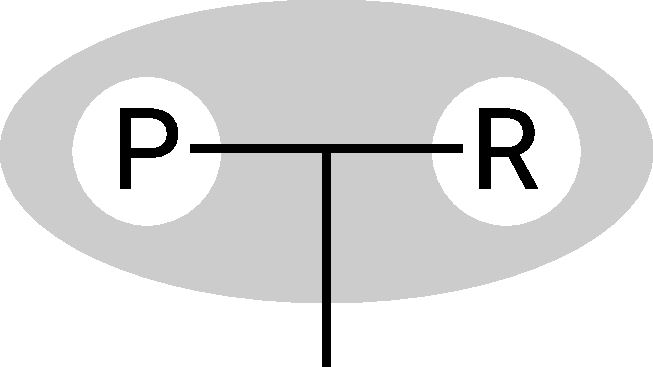
\includegraphics[height=3em]{gfx/related-work/existentialGraphExample1.pdf}}}
	\quad\Leftrightarrow\quad
	\exists\ a: P(a) \lor R(a)
\end{align*}
Wie schon die Begriffsschrift, sind Existenzgraphen syntaktisch minimal.
Direkt ausdrücken lässt sich lediglich \textit{UND}, der Existenzquantor und die Negation.
Ein weiterer Unterschied zur heutigen Prädikatenlogik ist die Beschreibung logischer Inferenzen.
Im Gegensatz zu den prädikatenlogischen Ersetzungsaxiomen, die auf der syntaktischen Struktur von logischen Ausdrücken operieren (z.~B. für Kommutativität), lassen sich die Ersetzungsaxiome für Existenzgraphen als Graphtransformationsregeln verstehen, die bestimmte Teilmengen der Knoten und Kanten eines Ausdrucks durch andere äquivalente Knoten- und Kantenmengen ersetzen.

\paragraph{Prädikatenlogik: Peano-Russell Notation (1910)}
Die zweidimensionalen Notationen wurde häufig kritisiert, da sie die lineare, algebraische Notation der symbolischen Logik von Boole und De Morgan verwarfen~\cite{Sluga1987}.
Freges Begriffsschrft und Peirces Existenzgraphen konnten sich daher nicht durchsetzen.
Peirces algebraische prädikatenlogische Notation hingegen, stieß auf größere Akzeptanz.
Giuseppe Peano hat auf deren Basis eine ähnliche Notation entwickelt, welche allerdings nicht die algebraischen Operatoren benutzt, damit sich logische Ausdrücke besser mit mathematischen Ausdrücken kombinieren lassen.
Bertrand Russell hat Peanos Notation anschließend in leicht abgewandelter Form in den \textit{Principia Mathematica}~\cite{Whitehead1910} benutzt.
Diese sog.~Peano-Russell-Notation ist im Wesentlichen identisch mit der modernen Schreibweise.

Trotz des Verschwindens der zweidimensionalen Notationen, finden sich noch heute Anlehnungen daran~\cite{WikiBegriffsschrift}.
So ist z.~B. die Negation $\lnot A$ auf Freges negierten Inhaltsstrich $\Fncontent A$ und der Ableitungsoperator $\vdash$ auf Freges Urteilsstrich mit angefügtem Inhaltsstrich $\Facontent$ zurückzuführen.

\subsection{Entwicklung maschineller Wissensrepräsentation}%
\label{sec:related:kr:history}

Die Idee Computer zur Lösung beliebiger Probleme zu benutzen ist nicht neu.
Da ein solches maschinelles Problemlösen die Verfügbarkeit von Hintergrundwissen über die Problemdomäne erfordert,
wurden Methoden zur Wissensrepräsentation immer im Zusammenhang mit Problemlösern erforscht.
So wie effiziente Datenstrukturen die Implementation effizienter Algorithmen ermöglichen, ermöglichen gute Wissensrepräsentationen die Implementation guter Problemlöser.
Was genau nun als ein guter Problemlöser verstanden wird, hat sich im Laufe der Jahre allerdings immer wieder verändert.

\paragraph{Universelle Problemlöser}
Einer der ersten maschinellen Problemlöser war der von Simon, Shaw und Newell 1955 entwickelte \textit{Logic Theorist} (LT).
LT war in der Lage logische Aussagen zu beweisen, indem er systematisch Ersetzungsaxiome auf eine gegebene Aussage angewandt hat, bis die gesuchte Lösung abgeleitet wurde.

Die Grundidee des LT haben Simon, Shaw und Newell 1959 im \textit{General Problem Solver} (GPS) erweitert.
Es wurden Heuristiken hinzugefügt, um den Suchraum geschickter zu durchlaufen.
GPS war ein universeller Problemlöser, konnte also jedes Problem lösen, das sich durch eine Menge von Horn-Klauseln ausdrücken lässt.
Zwar war es so theoretisch möglich Probleme aus diversen Domänen zu lösen, aufgrund der kombinatorischen Explosion war GPS alledings nicht zur Lösung komplexer praktischer Probleme geeignet.

\paragraph{Expertensysteme}
Aufgrund der Misserfolge universeller Problemlöser für praktische Probleme, hat die Forschung begonnen sich mehr auf die Entwicklung von Expertensystemen zu fokussieren.
Expertensysteme besitzen für gewöhnlich eine Wissensbasis in der domänenspezifisches Wissen in Form von Regeln und Fakten kodiert ist.
Eine sog.~Inferenzmaschine benutzt diese Regeln und Fakten um Probleme zu lösen.

\paragraph{Semantic Networks (1956)}
Die Idee, Graphen als Datenstruktur für Wissensbasen zu verwenden, taucht erstmal in den sog.~\textit{Semantic Networks} (zu dt.~semantische Netzwerke) auf.
Dieser Ansatz beschreibt Wissen als Menge von $(subject, predicate, object)$-Tripeln.
Es gibt darüber hinaus allerdings keine klaren Regeln, wie ein semantisches Netz strukturiert sein muss.
Semantische Netzwerke sind daher allenfalls als ein Oberbegriff für die große Vielfalt konkreter graphbasierter Wissensbasen zu verstehen.

\paragraph{Conceptual Graphs (1976)}
Wie genau mit Graphen komplexes Wissen beschrieben werden kann, das über eine reine Taxonomie hinaus geht, blieb bei semantischen Netzen unklar.
John F. Sowas \textit{Conceptual Graphs} (zu dt.~Konzeptgraphen) lösen dieses Problem.
Statt Wissen lediglich als eine einfache Menge von Beziehungen abzubilden, wird es als prädikatenlogischer Ausdruck verstanden.
Hierfür baut Sowa auf Peirces Existenzgraphen auf, die bis dahin weitestgehend unbeachtet waren.
\begin{align*}
	\vcenter{\hbox{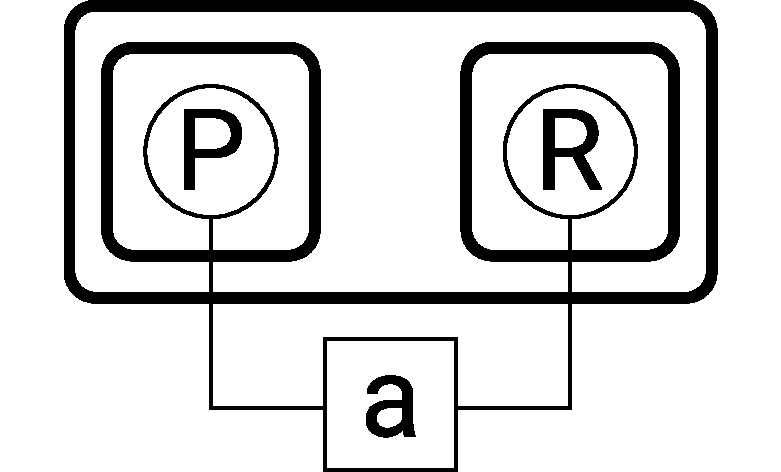
\includegraphics[height=4em]{gfx/related-work/conceptGraphExample1.pdf}}}
	\quad\Leftrightarrow\quad
	\exists\ a: P(a) \lor R(a)
\end{align*}
Dieser Ansatz erlaubt es komplexe Wissensbasen zu konstruieren, in denen nicht nur gespeichert werden kann, ob ein Konzept existiert, sondern auch, ob es nicht oder nur möglicherweise existiert.
Da Konzeptgraphen, so wie schon die Existenzgraphen, ein vollständiges und korrektes Logikkalkül sind, lassen sich zudem Inferenzregeln für sie definieren.
Der Vorteil hierfür einen Graphen statt eines prädikatenlogischen Ausdrucks zu verwenden ist, dass eine Graphstruktur einen deutlich effizienteren Zugriff auf gespeichertes Wissen ermöglicht.

\paragraph{Knowledge Graphs (1987)}
Der Begriff \textit{Knowledge Graph} (zu dt.~Wissensgraph) bezeichnete ursprünglich eine Klasse semantischer Netze, deren Relationsmenge formal spezifiziert ist.
Dies schränkt die Menge erlaubter Graphen ein und ermöglicht die Definition von Inferenzregeln, um Schlussfolgerungen aus einem gegebenen Graphen zu ziehen.
Im Laufe der Jahre ist die Grenze zwischen semantischen Netzen und Wissensgraphen allerdings immer weiter verschwommen, sodass die Bezeichnungen heute oft synonym verwendet werden.
Wissensgraphen und Konzeptgraphen müssen weiterhin unterschieden werden, da erstere oftmals Negation und Modalität nicht unterstützen.

\subsection{Aktuelle Wissensrepräsentationsprojekte}%
\label{sec:related:kr:today}

\subsubsection{Manuelle Ansätze}

\paragraph{Semantic Web}
Das sog.~\textit{Semantic Web} bezeichnet eine Menge von W3C-Standards, die das bestehende Web um eine formale Wissensbeschreibungssyntax erweitern.
Zentral ist dabei das \textit{Resource Description Framework} (RDF), mit dem sich beliebige Konzepte, auch Resourcen genannt, beschreiben und verknüpfen lassen.
Ziel ist es über die unstrukturierte Netzstruktur des bestehenden Webs, eine strukturierte, leicht maschniell verarbeitbare, Netzstruktur zu legen.
Durch die Anfragesprache \textit{SPARQL} ist es möglich Wissen aus diesem Netz auszulesen.
Das Web würde somit zu einem großen denzentralen Wissensgraphen.
Tim Berners-Lee beschreibt diese Idee als das ``Web 3.0''.
Obwohl die Technologien hierfür bereits seit Jahren existieren, sind bislang nur wenige Webseiten mit RDF-Tags annotiert.
Häufige Kritik ist, dass das Semantic Web zu viel theoretisches Hintergrundwissen über Wissensrepräsentationsverfahren erfordert, um für die meisten Webseitenbetreiber zugänglich zu sein.

\paragraph{WordNet}
Das \textit{WordNet} der Universität Princeton ist ein frei verfügbares lexikalisch-semantisches Netz für die englische Sprache, d.~h.\ ein semantisches Netz, welches die Bedeutung von Worten in Relation zueinander setzt.
Relationen werden dabei z.~B. für Synonyme, Hypernyme (Oberbegriffe) und Meronyme (Bestandteile) eingefügt.
Der Datenbestand des WordNets wird manuell gepflegt und resultiert aus der Kombination der Einträge verschiedener Wörterbücher.

\subsubsection{Automatisierte Ansätze}
Neben den manuellen Grapherzeugungsansätzen des Semantic Webs und des WordNets, gibt es diverse voll- und semiautomatische Ansätze.
Diese bauen die Graphstruktur selbstständig aus gegebenen Datenquellen auf.

\paragraph{NELL}
Das \textit{Never-Ending Language Learning} (NELL) System traviersiert selbstständig das Internet und fügt die gefundenen textuellen Informationen in einen Wissensgraphen ein.
Hierfür wird eine Kombination verschiedener Modelle verwendet, die regelmäßig angepasst wird.
Menschen können optional Feedback für die extrahierten Fakten geben, um die Inferenzqualität weiter zu verbessern.

\paragraph{Google Knowledge Graph}
Basierend auf den Ideen der in~\ref{sec:related:kr:history} vorgestellten Wissensgraphen, stellte Google 2012 eine eigene, ebenfalls \textit{Knowledge Graph} genannte, Wissensgraphtechnologie vor~\cite{Singhal2012}.
Sie wird benutzt, um Suchanfragen semantisch, statt per String-Matching, zu beantworten.
So können z.~B. zum Suchbegriff verwandte Ergebnisse angezeigt werden, selbst wenn es keine textuelle Ähnlichkeit zu jenem gibt.
Laut Googles Aussagen stammen die Quelldaten u.~a.\ aus Wikipedia Infoboxen, Wikidata und dem CIA World Factbook.
Da es sich hierbei, im Gegensatz zu NELL, primär um strukturierte Daten handelt, ist das automatisierte Einpflegen mit hoher Genauigkeit möglich.
Wie genau die Daten im Graph repräsentiert werden, ist nicht öffentlich bekannt.

\begin{figure}
	\begin{tikzpicture}
		\pgfplotstableread[col sep=comma] {data/related-work/knowledgeGraph.csv}\knowledgeGraphTrend%
		\begin{axis}[
			width=\textwidth,
			height=6cm,
			smooth,
			axis x line=bottom,
			axis line style={draw=none},
			ytick style={draw=none},
			ymin=0,
			ymax=100,
			ymajorgrids,
			ylabel={Popularität in \%},
			date coordinates in=x,
			date ZERO=2004-01-01,
			xmin={2004-01-01},
			xmax={2017-08-01},
			xticklabel={\month.\year},
			xtick={2004-01-01,2012-05-01,2017-08-01}
		]
			\addplot+[no markers,style=thick] table [x=month, y=popularity]{\knowledgeGraphTrend};
		\end{axis}
	\end{tikzpicture}
	\caption{Popularität des Begriffs ``knowledge graph'' (Quelle: Google Trends~\cite{Google2017})}\label{fig:related:kgTrend}
\end{figure}

\section{NLP-Werkzeuge}%
\label{sec:related:nlp}

Neben der Repräsentation von Wissen, ist auch die Verarbeitung natürlicher Sprache ein Kernbestandteil dieser Arbeit.
Hierfür existiert bereits eine Vielzahl von \textit{Natural Language Processing} (NLP) Werkzeugen.
Trotz dieser Vielfalt lassen sich Kernverarbeitungsschritte festmachen, die in den meisten Werkeugen verwendet werden.
\begin{enumerate}
	\item \textbf{Tokenization:}
		Oftmals einer der ersten Verarbeitungsschritte einer NLP Bibliothek.
		Eine Eingabezeichenkette wird dabei in eine Liste von Tokens zerlegt.
		Token sind u.~a. Wörter, Satzzeichen und numerische Literale.
		\[
			\text{``Today I'm testing myself.''}
			\rightarrow
			(\text{Today}, \text{I}, \text{'m}, \text{testing}, \text{myself}, \text{.})
		\]
	\item \textbf{Lemmatization:}
		Abbildung von Tokens auf ihre Lemmata (Grundformen).
		\[
			(\text{Today}, \text{I}, \text{'m}, \text{testing}, \text{myself}, \text{.})
			\rightarrow
			(\text {today}, \text{I}, \text{be}, \text{test}, \text{myself}, \text{.})
		\]
	\item \textbf{Part-of-speech Tagging:}
		Abbildung von Tokens auf ihre Wortarten (POS-Tags).
		\begin{center}
			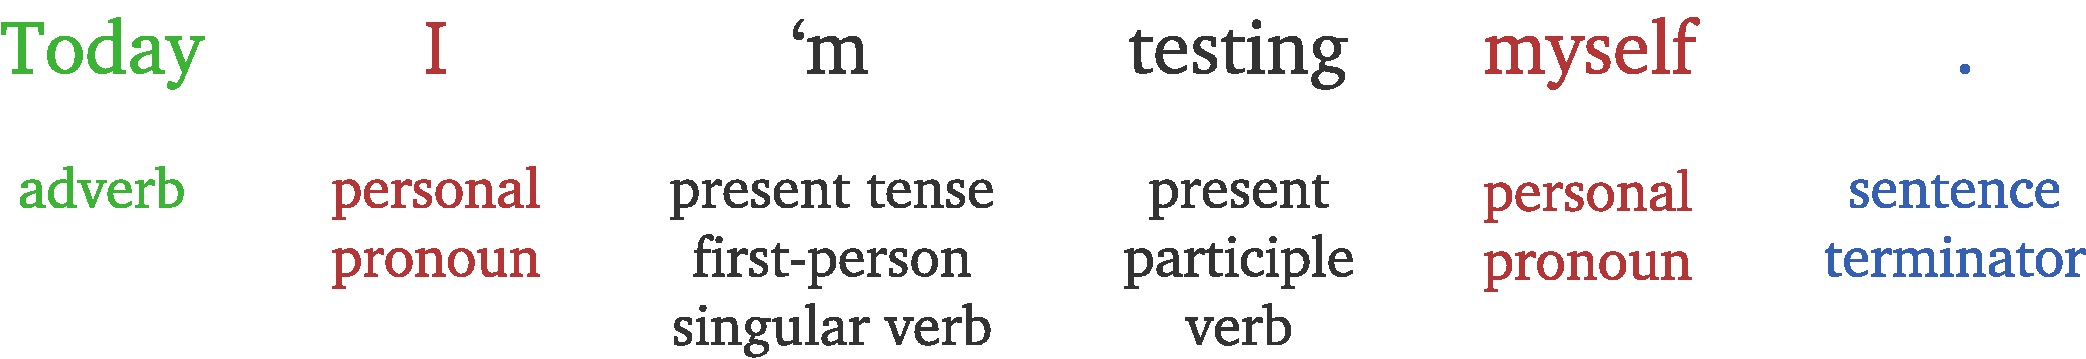
\includegraphics[height=4.5em]{gfx/related-work/posTaggingExample1.pdf}
		\end{center}
	\item \textbf{Named Entity Recognition:}
		Klassifizierung von Tokens in Kategorien wie z.~B. Person, Ort oder Zeitpunkt.
		\[
			({\color{gruen}\underbrace{\text{Today}}_{\text{date}}}, \text{I}, \text{'m}, \text{testing}, \text{myself}, \text{.})
		\]
	\item \textbf{Coreference Resolution:}
		Bestimmung von Token-Äquivalenzklassen, die jeweils auf das selbe Konzept verweisen (insbesondere Pronomina und ihr Antezedens).
		\begin{align*}
			(\text{Today}, \tikzmark{a}\text{\color{rot}I}, \text{'m},
			 \text{testing}, \text{\color{rot}my}\tikzmark{b}\text{\color{rot}self}, \text{.})
			\begin{tikzpicture}[overlay,remember picture]
				\draw[-,rot,shorten >=3pt,shorten <=3pt] (a.center) to[bend right] (b.center);
			\end{tikzpicture}
		\end{align*}
	\item \textbf{Dependency Parsing:}
		Eine auf den POS-Tags aufbauende syntaktische Analyse, welche die grammatikalischen Abhängigkeiten der Token untereinander ausgibt.
		Die Menge dieser Abhängigkeiten bildet einen Baum oder baumähnlichen Graphen, der \textit{Treebank} bzw.\ \textit{Dependency Graph} genannt wird.
		\begin{center}
			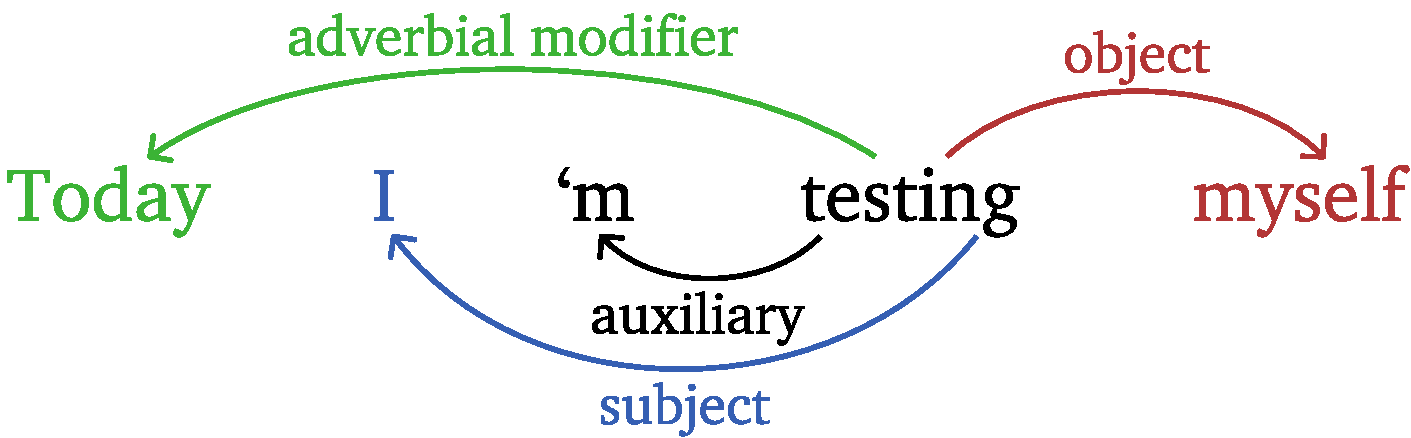
\includegraphics[height=5.5em]{gfx/related-work/depParseExample1.pdf}
		\end{center}
\end{enumerate}

Wie sich erkennen lässt, bauen die Verarbeitungsschritte sukzessive aufeinander auf und bilden eine Art Pipeline.
Dieses Pipeline-Modell findet sich auch in vielen NLP-Werkzeugen wieder.
Ein solches ist z.~B. das quelloffene Stanford~CoreNLP Projekt~\cite{Manning2014}\cite{CoreNLP}, welches u.~a. Module für alle der soeben vorgestellten Verarbeitungsschritte beinhaltet.
Ein alternatives NLP-Toolkit ist Apache~OpenNLP~\cite{OpenNLP};\@
es bietet ähnliche Module wie CoreNLP an.

\section{Wissensgraphkonstruktionsverfahren}%
\label{sec:related:kgc}

Wie in~\ref{sec:related:kr:today} gezeigt, gibt es diverse Ansätze um Graphen aus Daten zu konstruieren.
Da für das Thema dieser Arbeit insbesondere automatisierte Verfahren relevant sind, die mit unstrukurierten Daten, wie z.~B. natürlicher Sprache, umgehen können, werden diese im Folgenden näher beschrieben.

Üblicherweise arbeiten Wissensgraphkonstruktionsverfahren nicht direkt mit den unstrukturierten Eingabedaten, wie z.~B. den Inhalten von E-Mails,
sondern mit einer Knoten- bzw.\ Konzeptmenge und ggf.\ auch einer Kanten- bzw.\ Relationsmenge, die zuvor, z.~B. mittels eines in~\ref{sec:related:nlp} vorgestellten NLP-Verfahrens, aus den Rohdaten extrahiert wurden.
Die Wissensgraphkonstruktion ist somit äquivalent zum Problem der \textit{Link Prediction}, also dem Finden von Relationen zwischen den gegebenen Konzepten.
Die Link Prediction wiederum lässt sich als ein Problem des \textit{Statistical Relational Learnings} (SRL) auffassen.
In der Literatur finden sich im Wesentlichen drei Klassen von SRL-Verfahren~\cite{Nickel2016}, die auf verschiedenen Annahmen über die Korrelation der zu verknüpfenden Informationen basieren:
\begin{enumerate}
	\item \textbf{Latent Feature Models:}
		Alle Relationen werden als bedingt unabhängig angenommen, sofern bestimmte Eigenschaften über Subjekte und Objekte der Relationen gegeben sind.
	\item \textbf{Graph Feature Models:}
		Alle Relationen werden als bedingt unabhängig angenommen, sofern bestimmte Eigenschaften der Struktur des Graphen gegeben sind.
	\item \textbf{Markov Random Fields:}
		Es wird angenommen und erlaubt, dass alle Relationen lokale Abhängigkeiten voneinander haben können.
\end{enumerate}

\paragraph{Latent Feature Models}
Ein Beispiel für ein Latent Feature Modell ist das RESCAL-Verfahren~\cite{Nickel2013}, welches auf Tensorfaktorisierung basiert.
Die Grundidee dabei ist es, allen Entitäten $i$ einen Feature-Vektor $e_i \in \mathbb{R}^H$ zuzuordnen und für alle Relationen $k$ eine Gewichtsmatrix $W_k \in \mathbb{R}^{H \times H}$ zu finden.
Die Konfidenz in die Existenz einer Relation $i \xrightarrow{k} j$ wird durch $e_i^T\ W_k\ e_j$ beschrieben.
Diese Definition ermöglicht eine sehr schnelle Link Prediction, da lediglich ein Vektor-Matrix-Vektor-Produkt berechnet werden muss.
RESCAL liefert gute Ergebnisse, wenn die vorherzusagenden Relationen globale Abhängigkeiten aufweisen.
Lokal stark zusammenhängende Teilgraphen werden allerdings schlecht erkannt, da nur der Feature-Vektor und nicht die Nachbarschaft einer Entität berücksichtigt wird;
ein Beispiel hierfür sind symmetrische Relationen.
\[A \xrightarrow{\text{married to}} B \implies B \xrightarrow{\text{married to}} A\]

\paragraph{Graph Feature Models}
Komplementär zu den Latent Feature Modellen sind die Graph Feature Modelle.
Statt Entitäten in einen Feature-Raum einzubetten, wird hier die Nachbarschaft der Entitäten betrachtet.
Ein Beispiel hierfür ist der \textit{Path Ranking Algorithmus} (PRA)~\cite{Lao2011}. PRA ermittelt Relationen durch zufälliges Durchwandern des Graphen.
Um die Stärken der Latent Feature und Graph Feature Modelle zu kombinieren, wurden Hybrid-Modelle, wie z.~B. das \textit{Additive Relational Effects} (ARE) Verfahren~\cite{Nickel2014}, entwickelt, welches die Konfidenzen von RESCAL und PRA addiert.

\paragraph{Markov Random Fields}
Fundamental verschieden von diesen beiden Verfahren sind \textit{Markov Random Fields} (MRFs).
Hier sind prinzipiell Abhängigkeiten zwischen allen Relationen möglich, was MRFs sehr flexibel macht.
Da dies hinsichtlich der Laufzeit schnell impraktikabel wird, wird das Modell um einen Abhängigkeitsgraphen erweitert, der die Anzahl von betrachteten Abhängigkeiten reduziert.
Der Abhängigkeitsgraph darf dabei nicht mit dem Wissensgraphen verwechselt werden:
Ersterer beschreibt statistische Abhängigkeiten zwischen Klassen von Relationen, während letzterer Abhängigkeiten zwischen spezifischen Fakten beschreibt.
Zur Modellierung von Abhängigkeitsgraphen werden i.~d.~R. Kalküle verwendet, die an eine Prädikatenlogik erster Ordnung angelehnt sind.
Das Finden eines Wissensgraphen ist in diesem Modell äquivalent zum Lösen des MAX-SAT-Problems.
Wählt man ein Kalkül in dem die Atome stetig, also aus $[0, 1]$ statt aus $\{ 0, 1 \}$ sind, und Formeln zudem ausschließlich Disjunktionen und Negationen gemäß Łukasiewicz S-Norm enthalten, erhält man ein sog.\ \textit{Hinge-Loss-MRF}~\cite{Bach2013}\cite{Bach2015}, da die Loss-Funktion der Disjunktion in dieser S-Norm ein Hinge-Loss ist.

Ein konkretes Kalkül, welches sich zur Spezifikation von HL-MRFs eignet, ist die \textit{Probabilistic Soft Logic} (PSL)~\cite{Broecheler2010}\cite{Bach2015}.
MAX-SAT lässt sich für solche HL-MRFs effizient und parallelisierbar mit dem konvexen \textit{Alternating Direction Method of Multipliers} (ADMM) Optimierungsverfahren~\cite{Boyd2011} lösen.
In dessen ursprünglichen Form ist ADMM allerdings ausschließlich für offline Inferenz geeignet;
der Wissensgraph müsste also bei jeder Eingabe neu konstruiert werden.
Um dieses Problem zu lösen, wurde das \textit{Budgeted Online Collective Inference} (BOCI) Verfahren~\cite{Pujara2015} entwickelt.
BOCI nutzt Metadaten, die während der Ausführung von ADMM anfallen, um eine Bewertung für jedes Atom zu berechnen.
Die Bewertung eines Atoms beschreibt, wie groß die erwartete Wertveränderung beim Eintreffen neuer Informationen ist.
Kommen nun neue Informationen an, müssen diese ausschließlich zusammen mit den $m$ höchstbewerteten bereits existierenden Atomen betrachtet werden, die Werte aller anderen Atome werden fixiert.
Je höher das Budget $m$, desto höher ist die Qualität im Vergleich zu einer Neukonstruktion des Graphen.
Es wurde empirisch gezeigt, dass die Inferenzqualität mit BOCI oft nur unwesentlich schlechter ist als bei einer kompletten offline Inferenz.

Mittels ADMM und BOCI lässt sich PSL daher für die online Wissensgraphkonstruktion einsetzen.
Der Vorteil dieses Ansatzes gegenüber eines Latent Feature oder Graph Feature Modells ist, dass sich andere domänenspezifische Expertensysteme leicht in eine PSL Inferenz integrieren lassen.
PSL erlaubt nämlich die Inklusion von benutzerdefinierten Funktionen und Prädikaten.
Diese können benutzt werden, um z.~B. die Levenshtein-Distanz zweier Zeichenketten oder domänenspezifisches Hintergrundwissen, wie Distanz zwischen zwei namentlich genannten Orten, mit in die Entity Resolution einfließen zu lassen.
   % INCLUDE: related work
% !TEX root = ../main.tex
%
\chapter{System}
\label{sec:system}

\cleanchapterquote{Innovation distinguishes between a leader and a follower.}{Steve Jobs}{(CEO Apple Inc.)}

\Blindtext[2][1]

\section{System Section 1}
\label{sec:system:sec1}

\Blindtext[1][2]

\begin{figure}[htb]
	
\includegraphics[width=\textwidth]{gfx/Clean-Thesis-Figure}
	\caption{Figure example: \textit{(a)} example part one, \textit{(c)} example part two; \textit{(c)} example part three}
	\label{fig:system:example1}
\end{figure}

\Blindtext[1][2]

\section{System Section 2}
\label{sec:system:sec2}

\Blindtext[1][2]

\begin{figure}[htb]
	
\includegraphics[width=\textwidth]{gfx/Clean-Thesis-Figure}
	\caption{Another Figure example: \textit{(a)} example part one, \textit{(c)} example part two; \textit{(c)} example part three}
	\label{fig:system:example2}
\end{figure}

\Blindtext[2][2]

\section{System Section 3}
\label{sec:system:sec3}

\Blindtext[4][2]

\section{Conclusion}
\label{sec:system:conclusion}

\Blindtext[2][1]
         % INCLUDE: system
% !TEX root = ../my-thesis.tex
%
\chapter{Concepts: This text is here to test a very long title, to simulate the line break behavior, to show that an extremely long tilte also works}
\label{sec:concepts}

\cleanchapterquote{Users do not care about what is inside the box, as long as the box does what they need done.}{Jef Raskin}{about Human Computer Interfaces}

\Blindtext[2][1]

\section{Concepts Section 1}
\label{sec:concepts:sec1}

\Blindtext[2][2]

\section{Concepts Section 2}
\label{sec:concepts:sec2}

\Blindtext[3][2]

\section{Concepts Section 3}
\label{sec:concepts:sec3}

\Blindtext[4][2]

\section{Conclusion}
\label{sec:concepts:conclusion}

\Blindtext[2][1]
       % INCLUDE: concepts
% !TEX root = ../main.tex
% chktex-file 46
\chapter{Zusammenfassung}%
\label{sec:conclusion}

Abschließend wird nun zusammengefasst, inwiefern das in~\ref{sec:intro:goals} beschriebene Ziel einer erweiterbaren, parallelisierbaren Wissensgraph-Konstruktion aus Kommunikationsdaten erreicht wurde.
Hierfür werden in~\ref{sec:conclusion:review} die erreichten Teilziele betrachtet.
Anschließend wird in~\ref{sec:conclusion:todo} ein Ausblick auf Möglichkeiten der Weiterentwicklung des Systems gegeben.

\section{Rückblick}%
\label{sec:conclusion:review}

\begin{figure}[h]
	\centering
	
\includegraphics[width=0.65\textwidth]{gfx/conclusion/overview.pdf}
	\caption{Grober Aufbau des Konstruktionsverfahrens}\label{fig:conclusion:overview}
\end{figure}
In Kapitel~\ref{sec:text2kg} wurden Lösungen für die drei wesentlichen Teilprobleme Ontologie, Sprachverarbeitung und Grapherweiterung beschrieben.
Die drei Teillösungen bilden zusammen ein Konstruktionsverfahren, welches dem zu Anfang beschriebenen Aufbau entspricht.

\paragraph{Ontologie}
Die Wissensgraphontologie basiert auf Konzeptgraphen.
Im Gegensatz zu den Fakten-Tripel basierten semantischen Netzen, die lediglich beschreiben, welche Beziehungen zwischen Konzepten existieren, kann mittels Konzeptgraphen auch beschrieben werden, welche Beziehungen nicht, oder nur möglicherweise existieren.
Die konstruierten Wissensgraphen haben also eine deutlich höhere Ausdrucksstärke, als z.~B. NELL oder der Google~Knowledge~Graph.
Diese Ausdrucksstärke ist wichtig, um die Komplexität natürlichsprachlicher Aussagen abbilden zu können.

Damit den konstruierten Konzeptgraphen eine Semantik zugeordnet werden, muss die Semantik der verwendeten Relationen beschrieben werden.
Es wurde daher ein möglichst minimales Set von Relationen definiert~\tref{sec:text2kg:ontology:pred}, welches zur Beschreibung einer Vielzahl natürlichsprachlicher Aussagen geeignet ist.

Eine der in~\ref{sec:intro:goals} beschriebenen Anforderungen an das Konstruktionsverfahren ist die Erweiterbarkeit, d.~h.\ die prinzipielle Möglichkeit nicht natürlichsprachliche Eingaben einzufügen.
Konkret bedeutet dies, dass z.~B. ein Bild in denselben Wissensgraph eingefügt werden kann, in den auch Textnachrichten eingefügt werden.
Da die gewählten Konzeptgraph-Relationen nicht speziell für natürliche Sprache ausgelegt sind, ist dies prinzipiell möglich;
es gibt keine Relationen, die bestimmte grammatikalische Konstrukte oder Wortarten abbilden.
Wie die Integration anderer Eingabearten im Detail aussehen könnte, war jedoch nicht Teil der Aufgabenstellung und wurde daher nicht näher untersucht.

\paragraph{Sprachverarbeitung}
Für die Transformation einer Nachricht in einen Konzeptgraphen wurde das Stanford~CoreNLP Framework mit einer Menge von Transformationsregeln~\tref{sec:text2kg:nlp:transform} kombiniert, welche die von CoreNLP gefundenen Strukturen auf äquivalente Konzeptgraph-Strukturen abbilden.

\paragraph{Grapherweiterung}
Das Einfügen des aus einer Nachricht extrahierten Konzeptgraphen in einen bestehenden Wissensgraphen erfolgt mittels PSL.\@
Im Rahmen dieser Arbeit wurde PSL erstmals im Kontext einer Konzeptgraph-basierten Wissensgraph-Konstruktion eingesetzt.
Es wurde ein Set von PSL-Regeln~\tref{sec:text2kg:psl:inference} vorgestellt, welches den Einsatz in diesem Kontext exemplarisch aufzeigt.

Neben der Erweiterbarkeit war auch die Parallelisierbarkeit eines der in~\ref{sec:intro:goals} beschriebenen Ziele.
Durch die Wahl von PSL für die Grapherweiterung wurde diese Anforderung prinzipiell erfüllt.
Das für die Inferenz verwendete ADMM-Verfahren lässt sich gut verteilt implementieren.
In~\cite[Kapitel 10]{Boyd2011} wird beschrieben, wie sich ADMM mit verteilten Programmiermodellen, wie z.~B. MapReduce oder Pregel, implementieren lässt.
Aufbauend darauf, wird in~\cite{Lubell-Doughtie2013} eine Hadoop MapReduce-basierte Implementation vorgestellt.
PSL ist prinzipiell also für den Einsatz in Cluster-Umgebungen geeignet.
Die exemplarische verteilte PSL-Implementation \textit{foxPSL}~\cite{Magliacane2015} demonstriert dies.
In der im Rahmen dieser Arbeit erstellten Implementation wurde die PSL-Referenzimplementation verwendet, da diese am besten dokumentiert ist und die Geschwindigkeit für die verwendeten kleinen Datensets ausreichend ist.

Das Ziel ein erweiterbares, parallelisierbares Wissensgraph-Konstruktionsverfahren für Kommunikationsdaten zu konzipieren wurde somit prinzipiell erreicht.
Nichts desto trotz gibt es noch zahlreiche Möglichkeiten das vorgestellte Verfahren weiterzuentwickeln.

\section{Ausblick}%
\label{sec:conclusion:todo}

Im Folgenden wird ein Überblick über Möglichkeiten der Weiterentwickung und offen gebliebene Fragestellungen gegeben.

\paragraph{Verbessern der Testmethode}
Ein Problem bei der Konzeption des Verfahrens war der Umstand, dass es keine Kommunikationsdaten mit Referenzergebnissen gibt, anhand derer Änderungen am Verfahren bewertet werden können.
Die Qualität vieler Entscheidungen, wie z.~B. der Wahl der Regelgewichte, konnte daher nur auf Basis manuell durchgeführter, stichprobenartiger Tests bewertet werden.

Um dieses Problem zu lösen, könnte ein Kommunikationsdaten-Testset entwickelt werden, mit dem sich die Performance eines Wissensgraph-Konstruktionsverfahrens repräsentativ empirisch messen lässt.
Ein solches Datenset ist wichtig, um ein systematisches Weiterentwickeln des Verfahrens zu ermöglichen.
Das in dieser Arbeit verwendete Enron E-Mail Datenset ist potentiell ein guter Ausgangspunkt hierfür.
Zu klären ist, welche Art von Informationen die Referenzergebnisse enthalten und wie eine umfangreiche Menge solcher Referenzergebnisse konstruiert werden kann.

\paragraph{NLP-Phase}
Im vorgestellten Verfahren wird lediglich ein Teil der von CoreNLP extrahierten Informationen in Konzeptgraph-Strukturen übersetzt.
Durch die Integration bislang ungenutzter Abhängigkeitstypen ließe sich die Qualität der Ergebnisse, wie in~\ref{sec:evaluation:quality:results}~Anfrage~2 gezeigt, deutlich verbessern.

Außerdem sollte die verwendete Heuristik zur Übersetzung von natürlichsprachlicher Negation in negative Kontexte verbessert werden.
In~\ref{sec:evaluation:quality:results}~Anfrage~4 wird dies deutlich.
Ein Ansatz hierfür ist z.~B. das Nutzen des CoreNLP Natural Logic Annotators~\cite{MacCartney2007}, welcher u.~a.\ Quantoren, Negationen und die zugehörigen Scopes, d.~h.\ die modifizierten Token, erkennt.

\paragraph{PSL-Phase}
Die verwendeten domänenspezifischen Regeln und das domänenspezifische Vorwissen sind bislang sehr rudimentär.
In künftigen Arbeiten könnten vorhandene Wissensbasen, wie z.~B. NELL~\cite{Carlson2010} oder YAGO~\cite{YAGO}, in die PSL-Inferenz integriert werden.

Neben der Nutzung domänenspezifischen Wissens, besteht außerdem Verbesserungspotential bei der Nutzung von Kontexten in der Inferenz.
Bislang werden Kontexte nur benutzt, um die Richtung von $inst$-Relationen zu ermitteln.
Das Inferieren des $actual$-Attributs von Möglichkeitskontexten~\tref{sec:text2kg:ontology:modal} zur Bestimmung der Glaubwürdigkeit von Aussagen wäre z.~B. eine sinnvolle Erweiterung des Verfahrens.

\paragraph{Inferenz}
Wie~\treft{sec:evaluation:time} gezeigt hat, besteht noch Verbesserungsbedarf bei der Geschwindigkeit der PSL-Inferenz, bevor das Verfahren in der Praxis einsetzbar ist.
Um dies zu erreichen, ist die Kombination verschiedener Ansätze denkbar:
\begin{enumerate}
	\item Nutzen einer Cluster-fähigen ADMM-Implementation, statt der PSL-Referenz\-implementation.
		Hierfür könnte z.~B. die zuvor erwähnte Hadoop MapReduce Implementation~\cite{Lubell-Doughtie2013} oder foxPSL~\cite{Magliacane2015} verwendet werden.
	\item Weiterentwicklung von BOCI, sodass wachsende Eingabemengen unterstützt werden.
		Bereits im ursprünglichen Paper~\cite[Abschnitt 6]{Pujara2015} wird dies als offene Fragestellung für folgende Arbeiten genannt.
		Mittels des Inferenz-Budgets könnte dann die Inferenzdauer nahezu beliebig verringert werden, sofern dafür eine entsprechende Verschlechterung der Inferenzqualität hingenommen wird.
	\item Effizienterer Umgang mit transitiven Relationen.
		Bei der Inferenz werden $inst$-Atome aufgrund der Transitivität von $inst$ instanziiert.
		Während der Inferenz sind diese Atome wichtig, sie werden momentan allerdings auch Teil des Wissensgraphen.
		Das Entfernen dieser redundanten $inst$-Atome, würde die Kantenanzahl des in~\ref{sec:evaluation:time} konstruierten Graphen um mehr als 75\% verringern.
		Während der Inferenz würden die transitiven $inst$-Relationen dann nur temporär instanziiert.
		Inwiefern durch eine derartige Erweiterung der PSL-Inferenz neben der Graph-Größe auch die Inferenzdauer verringert werden kann, ist zu untersuchen.
\end{enumerate}

Wie soeben gezeigt, gibt es viele Möglichkeiten das vorgestellten Wissensgraph-Konstruktionsverfahren weiterzuentwickeln.
Diese Arbeit ist daher primär als ein Ausgangspunkt zu verstehen, der zeigt, dass die Kombination von Konzeptgraphen, NLP und PSL prinzipiell für die automatisierte Konstruktion von Wissensgraphen geeignet ist.
Aufbauend auf dieser Grundidee könnte in künftigen Arbeiten ein in der Praxis einsetzbares Verfahren entwickelt werden.
     % INCLUDE: conclusion

% --------------------------
% Back matter
% --------------------------
\appendix\cleardoublepage
% !TEX root = ../my-thesis.tex
%
\chapter{Example Appendix}
\label{sec:appendix}

\Blindtext[1][1]

\section{Appendix Section 1}
\label{sec:appendix:sec1}

\Blindtext[1][1]

\begin{table}[h]
	\begin{tabularx}{\textwidth}{X | X | X}
		%\hline
		Alpha		& Beta			& Gamma			\\ \hline
		0			& 1				& 2				\\ \hline
		3			& 4				& 5				\\ %\hline
	\end{tabularx}
	\label{tab:table1}
	\caption{This is a caption text.}
\end{table}

\section{Appendix Section 2}
\label{sec:appendix:sec2}

\Blindtext[1][1]

\begin{table}[h]
	\begin{tabularx}{\textwidth}{X | X | X}
		%\hline
		Alpha		& Beta			& Gamma			\\ \hline
		0			& 1				& 2				\\ \hline
		3			& 4				& 5				\\ %\hline
	\end{tabularx}
	\label{tab:table2}
	\caption{This is a caption text.}
\end{table}

\Blindtext[1][2]
       % INCLUDE: appendix
%
{%
\setstretch{1.1}
\renewcommand{\bibfont}{\normalfont\small}
\setlength{\biblabelsep}{0pt}
\setlength{\bibitemsep}{0.5\baselineskip plus 0.5\baselineskip}
\printbibliography[nottype=online]
\printbibliography[heading=subbibliography,title={Webpages},type=online,prefixnumbers={@}]
}
\cleardoublepage

\listoffigures
\cleardoublepage

\listoftables
\cleardoublepage

% !TEX root = ../main.tex
%
\pagestyle{empty}
\hfill
\vfill
\pdfbookmark[0]{Colophon}{Colophon}
\section*{Colophon}

This thesis was typeset with \LaTeXe.
It uses the \textit{Clean Thesis} style developed by Ricardo Langner.
The design of the \textit{Clean Thesis} style is inspired by user guide documents from Apple Inc.

Download the \textit{Clean Thesis} style at \url{http://cleanthesis.der-ric.de/}.

\cleardoublepage

% !TEX root = ../main.tex
%
%************************************************
% Declaration
%************************************************
\pdfbookmark[0]{Declaration}{Declaration}
\chapter*{Declaration}
\label{sec:declaration}
\thispagestyle{empty}

You can put your declaration here, to declare that you have completed your work solely and only with the help of the references you mentioned.

\bigskip

\noindent\textit{\thesisUniversityCity, \thesisDate}

\smallskip

\begin{flushright}
	\begin{minipage}{5cm}
		\rule{\textwidth}{1pt}
		\centering\thesisName
	\end{minipage}
\end{flushright}

%*****************************************
%*****************************************

\clearpage
\newpage
\mbox{}

% **************************************************
% End of Document CONTENT
% **************************************************
\end{document}
